
\chapter{\IfLanguageName{dutch}{Proof of Concept}{Proof of Concept}}%

\label{ch:proof-of-concept}

\section{Opbouw scenario's}

Om de \textit{Swift OpenAPI Generator} grondig te testen, concentreren we ons op een specifiek onderwerp: een boekenverlanglijst. Dit overkoepelende idee is onderverdeeld in kleinere scenario’s om het beter te kunnen uitwerken en de mogelijkheden van de \textit{Swift OpenAPI Generator} te gaan testen. 

\begin{itemize}
  \item	Scenario 1: gedeelde lijst van boeken met databaseconnectie
  \item	Scenario 2: back-end logica toevoegen voor \textit{logging}, \textit{metrics} en validatie. 
  \item Scenario 3: toevoegen van authenticatie
  \item Scenario 4: \textit{client} van de server aanmaken
  \item Scenario 5: aanpasbaarheid van back-end achter dat er een \textit{client} is toegevoegd
\end{itemize}

\section{Scenario 1: Gedeelde lijst van boeken met databaseconnectie}
Gebruikers hebben toegang tot een gedeelde lijst van boeken, waar ze informatie over elk boek kunnen bekijken en boeken kunnen gaan toevoegen en aanpassen. Deze lijst is toegankelijk voor alle gebruikers en maakt verbinding met een database om de boeken op te slaan en op te halen. 

\subsection{Technische doelstellingen}
De technische doelstellingen omvatten verschillende belangrijke aspecten. Allereerst moet er een OpenAPI-document gecreërd worden dat alle vereiste requestmethoden omvat, zoals POST, CREATE, UPDATE, GET en GET / ID.  Dit document bevat een gedetailleerde opsomming van hoe verzoeken geformuleerd en verwerkt moeten worden. Het is opgesteld volgens de OpenAPI-specificaties. Daarnaast is het essentieel om een stabiele en efficiënte databaseverbinding tot stand te brengen, zodat de nodig boekgegevens kunnen opslaan en ophalen. 

Eenmaal verbonden met de database, moet de \textit{handler} uitgewerkt worden. Deze \textit{handler} is verantwoordelijk is voor het verwerken van alle inkomende verzoeken. Hierbij wordt de nodige logica toegevoegd om aan elke type verzoek correct te kunnen voldoen. Dit omvat het verwerken van verzoeken voor het toevoegen, bijwerken en opvragen van boekgegevens, evenals het ophalen van specifieke boeken op basis van hun unieke ID.


\subsubsection{Aanmaken van OpenAPI document}

Een correcte syntax is essentieel bij het opstellen van een OpenAPI-document, aangezien zelfs een kleine fout de interpretatie van de generator kan beïnvloeden. Om dergelijke fouten te voorkomen, Zijn de OpenAPI-document gemaakt in VScode met behulp van de extensie 'vscode-openapi-viewer'. 

In een OpenAPI-document begint men met het specificeren van de versie, gevolgd door eventuele aanvullende informatie in de 'info'-sectie. Vervolgens worden de servers gedefinieerd om aan te geven op welke URL de API zal draaien. Pas daarna worden de paden en \textit{endpoints} van de API gespecificeerd.

Helemaal onderaan, na de specificatie van de paden en \textit{endpoints}, volgt de sectie voor het definiëren van de \textit{components}. Deze \textit{components} zijn herbruikbare elementen binnen het OpenAPI-document. Dit kunnen schema's voor gegevensstructuren, parameters, en antwoorden op verzoeken zijn. Door componenten te gebruiken, kunnen we duplicatie verminderen en consistentie waarborgen in het hele document.

\begin{lstlisting}[caption=openapi.yml file]
openapi: 3.1.0
info:
  title: Books API
  version: 1.0.0
servers:
  - url: 'http://localhost:8080/api'

paths:
  /books:
    get:
      operationId: getAllBooks
      summary: Get all books

      description: Returns a list of all books
      responses:
        '200':
          description: A list of books
           content:
             application/json:
               schema:
                 type: array
                 items:
                   $ref: '#/components/schemas/Book'
    post:
      operationId: createBook
      summary: Create a new book
        description: Creates a new book
        requestBody:
          content:
            application/json:
              schema:
                $ref: '#/components/schemas/Book'
        responses:
          '201':
            description: The created book
            content:
              application/json:
                schema:
                  $ref: '#/components/schemas/Book'
  /books/{id}:
    get:
      operationId: getById
      summary: Get a book by ID
      description: Returns a book with the specified ID
      parameters:
        - name: id
          in: path
          description: The ID of the book
          required: true
          schema:
            type: string
      responses:
        '200':
           description: A book
           content:
             application/json:
               schema:
                 $ref: '#/components/schemas/Book'
        '404':
          description: Book not found
    put:
      operationId: updateBook
      summary: Update a book by ID
      description: Updates a book with the specified ID
      parameters:
        - name: id
          in: path
          description: The ID of the book
          required: true
          schema:
            type: string
      requestBody:
        content:
          application/json:
            schema:
              $ref: '#/components/schemas/Book'
      responses:
        '200':
          description: The updated book
          content:
            application/json:
              schema:
                $ref: '#/components/schemas/Book'
components:
  schemas:
    Book:
      type: object
      properties:
        id:
          type: string
          description: The ID of the book
        title:
          type: string
          description: The title of the book
        author:
          type: string
          description: The author of the book
required:
  - id
  - title
  - author

\end{lstlisting}

\begin{lstlisting}[caption=openapi-generator-config.yaml file]
    generate:
    - types
    - server
\end{lstlisting}


\subsubsection{Verbinding met database}

Bij de eerste poging om verbinding te maken met de database, werd er het voorbeeld gebruikt dat beschikbaar was op de Git-repository van de \textit{Swift OpenAPI Generator}. Maar al snel werd duidelijk dat dit voorbeeld veel te \textit{low-level} was. Het maakt de code complex en ingewikkeld, waardoor het lastig was om een efficiënte database verbinding tot stand te brengen die kon herbruikt worden.  
Er werd over gegaan naar meer vertrouwde methoden. Er werd geprobeerd om de connectie op te zetten zoals gebruikelijk is bij het ontwikkelen van back-end-systemen. 

Zo is de database toegevoegd aan de de \textit{main server} van de applicatie. Zodat deze onmiddellijk wordt opgezet als de applicatie runt. Om de database operationeel te maken en de benodigde tabellen toe te voegen, is er gebruik gemaakt van \textit{migrations}. Door \textit{migrations} te gebruiken, kan er gemakkelijk wijzigingen in de databasestructuur doorgevoerd worden en deze synchroniseren met de applicatiecode. Dit garandeert een consistente en betrouwbare databaseconfiguratie.
\begin{lstlisting}[caption=Migration file]
   import Fluent
   struct CreateBooks: AsyncMigration {
       func prepare(on database: FluentKit.Database) async throws {
           return try await database.schema("books")
           .id()
           .field("title", .string, .required)
           .field("author", .string)
           .create()
       }
       
       func revert(on database: FluentKit.Database) async throws {
           try await database.schema("books").delete()
       }
   } 
\end{lstlisting}

Daarnaast zijn er  models gemaakt voor de gegevens die in de database worden opgeslagen. Dit is gedaan omdat de standaard datatypen van een OpenAPI-document niet rechtstreeks aan de database kunnen worden toegevoegd. Dit betekent dat wanneer er een verzoek wordt gedaan aan de applicatie, de gegevens die worden ontvangen eerst moet worden aangepast naar het juiste gegevenstype.

\begin{lstlisting}[caption=Model file]
final class Book: Model, Content {
    static let schema = "books"
    @ID(key: .id)
    var id: UUID?
    @Field(key: "title")
    var title : String
    @Field(key: "author")
    var author : String
    
    init() { }
    
    init(id: UUID? = nil, title: String, author: String) {
        self.id = id
        self.title = title
        self.author = author
    }
}
\end{lstlisting}

In traditionele back-end systemen is het mogelijk om de database op te halen aan de hand van het \textit{Request} dat je ontvangt, maar tegen initiële verwachtingen in werkte dit niet met de \textit{Swift OpenAPI Generator}. Dit komt doordat de Swift OpenAPI generator zelf een APIProtocol heeft, wat een extra laag van complexiteit toevoegt. Concreet betekent dit dat de gebruikelijke methoden om de database op te halen niet functioneerden zoals anders. Om dit op te lossen, wordt er simpelweg de database door gegeven van de server aan de \textit{handler}. Dit was een effectieve oplossing die ervoor zorgde dat de database toegankelijk was zonder te interfereren met de werking van de \textit{Swift OpenAPI Generator}.

\begin{lstlisting}[caption=booksServiceServer file]
@main struct booksServiceServer {
    static func main() async throws {
        
        let app = Vapor.Application()
        app.databases.use(DatabaseConfigurationFactory.postgres(configuration: .init(
        hostname: Environment.get("DATABASE_HOST") ?? "localhost",
        port: Environment.get("DATABASE_PORT").flatMap(Int.init(_:)) ?? SQLPostgresConfiguration.ianaPortNumber,
        username: Environment.get("DATABASE_USERNAME") ?? "vapor_username",
        password: Environment.get("DATABASE_PASSWORD") ?? "vapor_password",
        database: Environment.get("DATABASE_NAME") ?? "vapor_database",
        tls: .prefer(try .init(configuration: .clientDefault)))
        ), as: .psql)
        
        app.migrations.add(CreateBooks())
        try app.autoMigrate().wait()
        
        let transport = VaporTransport(routesBuilder: app)
        let handler = Handler(app: app)
        try handler.registerHandlers(on: transport, serverURL: URL(string: "/api")!)
        try await app.execute()
    }

\end{lstlisting}

\subsubsection{Toevoegen van de \textit{handler}}
Nadat de verbinding met de database tot stand is gebracht, is het noodzakelijk om de verzoeken vanuit het OpenAPI-document nog te verwerken. Deze verwerking wordt doorgaans uitgevoerd in de \textit{handler} van de applicatie. De \textit{handler} fungeert als een tussenliggende laag tussen de ontvangen verzoeken en de daadwerkelijke verwerking ervan.

Binnen de \textit{handler} worden de ontvangen verzoeken geanalyseerd, gevalideerd en doorgegeven aan de database. Dit omvat vaak het interpreteren van de gegevens in het verzoek, het oproepen van de bijbehorende methoden of services om de gevraagde acties uit te voeren en het afhandelen van eventuele fouten of uitzonderingen die zich tijdens dit proces kunnen voordoen. Het ontwikkelen van een efficiënte \textit{handler} is van groot belang want zonder deze \textit{handler} zal de back-end niet kunnen functioneren.

\begin{lstlisting}[caption=handler file]
import OpenAPIRuntime
import OpenAPIVapor
import Vapor
import Fluent
import FluentPostgresDriver

struct Handler: APIProtocol { 
    let app : Application
    init(app: Application) {
        self.app = app
    }

    func getAllBooks(_ input: Operations.getAllBooks.Input) async throws -> Operations.getAllBooks.Output {
        let books = try await Book.query(on: app.db).all()
        
        var booksArray: Array<Components.Schemas.Book> = []
        books.forEach { book in
            booksArray.append(Components.Schemas.Book(id: "\(String(describing: book.id))", title: book.title, author: book.author))
        }
        return .ok(.init(body: .json(booksArray)))
    }
    
    func getById(_ input: Operations.getById.Input) async throws -> Operations.getById.Output {
        let id = UUID(uuidString: input.path.id)
        guard let book = try await Book.find(id, on: app.db) else {
            throw Abort(.notFound)
        }
        
        return .ok(.init(body: .json(Components.Schemas.Book(id: "\(String(describing: book.id))", title: book.title, author: book.author))))
    }

    func createBook(_ input: Operations.createBook.Input) async throws -> Operations.createBook.Output {
        guard case .json(let bookInput) = input.body else {
            fatalError()
        }
        
        let id = UUID(uuidString: bookInput.id)
        var book = Book(id: id, title: bookInput.title, author: bookInput.author)
        try await book.save(on: app.db)
        
        let bookapi: Components.Schemas.Book
        switch input.body {
            case .json(let json): bookapi = json
            case .none:
            bookapi = .init(id: "", title: "", author: "")
            break
        }
        
        return .created(.init(body: .json(bookapi)))
    }
    
    func updateBook(_ input: Operations.updateBook.Input) async throws -> Operations.updateBook.Output {
        guard case .json(let bookInput) = input.body else {
            logger.debug("Something went wrong with the Input.body")
            fatalError()
        }
        let id = UUID(uuidString: bookInput.id)
        guard let bookDb = try await Book.find(id, on: app.db) else {
            throw Abort(.notFound)
        }
        bookDb.id = UUID(uuidString: bookInput.id)
        bookDb.title = bookInput.title
        bookDb.author = bookInput.author
        
        try await bookDb.update(on: app.db)
        
        let updatedBook: Components.Schemas.Book
        switch input.body {
            case .json(let json): updatedBook = json
            case .none:
            updatedBook = .init(id: "", title: "", author: "")
            break
        }
        return .ok(.init(body: .json(updatedBook)))
    }
}

\end{lstlisting}

\section{Scenario 2: back-end logica toevegen voor \textit{logging}, \textit{metrics} en validatie}

Het tweede scenario is minder direct gerelateerd aan de applicatie zelf, maar richt zich meer op de logica die in de back-end plaatsvindt. De belangrijkheid van deze back-end logica kan niet worden onderschat, aangezien het essentieel is voor verschillende kritische functies. Dit omvat het bijhouden van fouten en gebeurtenissen, het meten van de prestaties van de applicatie en het valideren van de invoer om de integriteit en betrouwbaarheid van de gegevens die door de applicatie worden verwerkt te waarborgen.

\subsection{Technische doelstellingen}

\textit{Logging}, \textit{metrics} en validatie zijn onmisbare technische aspecten in de back-end van een applicatie. Ze vervullen elk een cruciale rol bij het waarborgen van de betrouwbaarheid, prestaties en integriteit van de applicatie.

\textit{Logging} legt de belangrijke gebeurtenissen en fouten vast die zich voordoen tijdens de uitvoering van de applicatie. Dit omvat het registreren van informatie zoals gebruikersacties, systeemgebeurtenissen, foutmeldingen en meer. Door \textit{logging} toe te voegen kunnen ontwikkelaars gemakkelijker een probleem opsporen en debuggen, wat cruciaal is voor het onderhouden van een gezonde applicatie. 

Aan de andere kant omvatten \textit{metrics} meetbare informatie over de prestaties en het gedrag van de applicatie. Dit kan variëren van de verwerkingstijd van verzoeken en geheugengebruik tot CPU-gebruik en het aantal gebruikers. \textit{Metrics} worden vaak samengevoegd en in kaart gebracht met monitoringssystemen zoals DataDog, Grafana en Prometheus. Het gebruik van \textit{metrics} geeft inzicht in de prestatie van de applicatie, helpt bij het identificeren van zwakke punten en maatschappelijke problemen, en stelt ontwikkelaars in staat proactief actie te ondernemen om de diensten te verbeteren. 

Tot slot, validatie richt zich op het controleren van de geldigheid en integriteit van de gegevens die door de applicatie worden verwerkt. Dit omvat het valideren van invoer van gebruikers om ervoor te zorgen dat deze voldoet aan verwachte criteria, zoals datums, geldige e-mailadressen, numerieke waarden en meer. Door validatie te voorzien kunnen ontwikkelaars potentiële fouten en inconsistentie voorkomen, Hierdoor zal de betrouwbaarheid en bruikbaarheid van de applicatie verbeteren.

\subsubsection{Implementeren van \textit{logging} met SwiftLog}
De \textit{wift OpenAPI-generator} biedt al enkele standaardlogs, maar als er meer \textit{logging} nodig zijn, is het mogelijk om Swiftlog te integreren. In dit project heeft men dit volledig uitgewerkt volgens de gebruikelijke methode om \textit{logging} toe te voegen aan een back-end applicatie. Het proces verliep soepel en de \textit{logging} functioneert zoals verwacht, waardoor het mogelijk is om een gedetailleerder inzicht te verkrijgen in de werking van de applicatie.
Bovendien bestaat er de mogelijkheid om \textit{logging} toe te voegen via een \textit{middleware}, wat een handige optie is om te verkennen. Deze \textit{middleware} is beschikbaar op de \textit{ OpenAPI-generator} GitHub-pagina, waardoor het gemakkelijk is om deze functionaliteit toe te voegen aan een project. Met deze aanvullende opties kan de \textit{logging}-functionaliteit van de \textit{Swift}-applicatie verder worden aangepast en geoptimaliseerd naar specifieke behoeften.

\begin{lstlisting}[caption=booksServiceServer file]
@main struct booksServiceServer {
    static func main() async throws {
        
        let app = Vapor.Application()
        var logger : Logger =  .init(label: "BookService")
        logger.logLevel = .trace
        
        logger.info("Setting up database");
        app.databases.use(DatabaseConfigurationFactory.postgres(configuration: .init(
        hostname: Environment.get("DATABASE_HOST") ?? "localhost",
        port: Environment.get("DATABASE_PORT").flatMap(Int.init(_:)) ?? SQLPostgresConfiguration.ianaPortNumber,
        username: Environment.get("DATABASE_USERNAME") ?? "vapor_username",
        password: Environment.get("DATABASE_PASSWORD") ?? "vapor_password",
        database: Environment.get("DATABASE_NAME") ?? "vapor_database",
        tls: .prefer(try .init(configuration: .clientDefault)))
        ), as: .psql)
        logger.info("Database connection secure");
        logger.info("Setting up migrations...");
        app.migrations.add(CreateBooks())
        app.migrations.add(CreateUser())
        app.migrations.add(CreateUserToken())
        try app.autoMigrate().wait()
        logger.info("migrations successfull added")
        
        
        let transport = VaporTransport(routesBuilder: app)
        let handler = Handler(app: app, logger: logger)
        try handler.registerHandlers(on: transport, serverURL: URL(string: "/api")!)
        try await app.execute()
    }
}

\end{lstlisting}

\begin{lstlisting}[caption=handler file]
struct Handler: APIProtocol {
    var logger : Logger =  .init(label: "my-Handler")
    let app : Application
    init(app: Application , logger: Logger ) {
        self.app = app
        
    }
    
    func getAllBooks(_ input: Operations.getAllBooks.Input) async throws -> Operations.getAllBooks.Output {
        let books = try await Book.query(on: app.db).all()
        logger.info("successfull GET-request to database")
        
        var booksArray: Array<Components.Schemas.Book> = []
        books.forEach { book in
            booksArray.append(Components.Schemas.Book(id: "\(String(describing: book.id))", title: book.title, author: book.author))
        }
        logger.info("Converted books of database to return object")
        return .ok(.init(body: .json(booksArray)))
        
    }
    
    func getById(_ input: Operations.getById.Input) async throws -> Operations.getById.Output {
        let id = UUID(uuidString: input.path.id)
        guard let book = try await Book.find(id, on: app.db) else {
            logger.debug("Can't find Book in database!")
            throw Abort(.notFound)
        }
        
        return .ok(.init(body: .json(Components.Schemas.Book(id: "\(String(describing: book.id))", title: book.title, author: book.author))))
        
    }

    func createBook(_ input: Operations.createBook.Input) async throws -> Operations.createBook.Output {
        guard case .json(let bookInput) = input.body else {
            logger.debug("Something went wrong with the Input.body")
            fatalError()
        }
        
        let id = UUID(uuidString: bookInput.id)
        var book = Book(id: id, title: bookInput.title, author: bookInput.author)
        try await book.save(on: app.db)
        
        let bookapi: Components.Schemas.Book
        switch input.body {
            case .json(let json): bookapi = json
            case .none:
            bookapi = .init(id: "", title: "", author: "")
            break
        }
        
        return .created(.init(body: .json(bookapi)))
    }
    
    func updateBook(_ input: Operations.updateBook.Input) async throws -> Operations.updateBook.Output {
        guard case .json(let bookInput) = input.body else {
            logger.debug("Something went wrong with the Input.body")
            fatalError()
        }
        let id = UUID(uuidString: bookInput.id)
        guard let bookDb = try await Book.find(id, on: app.db) else {
            throw Abort(.notFound)
        }
        bookDb.id = UUID(uuidString: bookInput.id)
        bookDb.title = bookInput.title
        bookDb.author = bookInput.author
        
        try await bookDb.update(on: app.db)
        
        let updatedBook: Components.Schemas.Book
        switch input.body {
            case .json(let json): updatedBook = json
            case .none:
            updatedBook = .init(id: "", title: "", author: "")
            break
        }
        return .ok(.init(body: .json(updatedBook)))
    
    }    
}

\end{lstlisting}

\subsubsection{Implementeren van Metrics}
Met behulp van de \textit{middleware} die beschikbaar is op de \textit{Swift OpenAPI Generator} GitHub-pagina, was het zeer eenvoudig om \textit{Metrics} toe te voegen aan de applicatie.  Door \textit{metrics} toe te voegen via een \textit{middleware} biedt dit een grote flexibiliteit en aanpasbaarheid. De \textit{metrics} kunnen op maat worden gemaakt naar uw specifieke behoeften en vereisten, waardoor een uitgebreide set aan meetgegevens kan worden verzameld die relevant is voor uw applicatie.

\begin{lstlisting}[caption=booksServiceServer file]
@main struct booksServiceServer {
    static func main() async throws {
        let registry = PrometheusCollectorRegistry()
        MetricsSystem.bootstrap(PrometheusMetricsFactory(registry: registry))
        let app = Vapor.Application()
        var logger : Logger =  .init(label: "BookService")
        logger.logLevel = .trace
        
        ……
        
        app.get("metrics") { request in
            var buffer: [UInt8] = []
            buffer.reserveCapacity(1024)
            registry.emit(into: &buffer)
            return String(decoding: buffer, as: UTF8.self)
        }
        
        
        let transport = VaporTransport(routesBuilder: app)
        let handler = Handler(app: app, logger: logger)
        try handler.registerHandlers(on: transport, serverURL: Servers.server1(), middlewares: [MetricsMiddleware(counterPrefix: "BooksServiceServer")])
        
        let host = ProcessInfo.processInfo.environment["HOST"] ?? "localhost"
        let port = ProcessInfo.processInfo.environment["PORT"].flatMap(Int.init) ?? 8080
        
        app.http.server.configuration.address = .hostname(host, port: port)
        try await app.execute()
    }
}

\end{lstlisting}

\subsubsection{Implementeren van validatie}
in de back-end maakt men gebruik van models. Aanvankelijk dacht men deze models te kunnen gebruiken om de gegevens te valideren. Echter al snel werd duidelijk dat dit niet ging lukken. Want deze validaties werken volgens een \textit{request} die bij de \textit{Swift OpenAPI Generator} niet gebruikt wordt. 

Een andere poging was om de validatie uit te voeren op basis van het format of de string zoals gespecificeerd in het OpenAPI-document. Het OpenAPI-document beschrijft de verwachte structuur en eigenschappen van de invoerparameters. Deze benadering leek veelbelovend omdat het een gestandaardiseerde manier bood om de geldigheid van het verzoek te waarborgen. Tegen initiële verwachtingen in, werkt deze methode niet met de \textit{Swift OpenAPI Generator}, wat het integratieproces bemoeilijkte en uiteindelijk niet haalbaar maakte.

Ten slotte is er  gekozen voor een meer pragmatische aanpak door handmatige validatie uit te voeren in de \textit{handler} voordat de gegevens werden opgeslagen in de database. Dit betekende dat de specifieke validatielogica rechtstreeks in de code van de \textit{handler} is implementeerd om ervoor te zorgen dat het verzoek voldeed aan de vereiste criteria voordat het wordt verwerkt. Hoewel dit een meer arbeidsintensieve oplossing was, bleek het effectief te zijn en te voldoen aan onze validatiebehoeften. Door de validatiestappen direct in de verwerkingslogica op te nemen, kan er nauwkeurige en betrouwbare gegevensverwerking gegarandeerd worden voordat deze werd opgeslagen in de database.

\begin{lstlisting}[caption=handler file]
struct Handler: APIProtocol {
    
    var logger : Logger =  .init(label: "my-Handler")
    let app : Application
    
    init(app: Application , logger: Logger ) {
        self.app = app
    }
    …
    
    func createBook(_ input: Operations.createBook.Input) async throws -> Operations.createBook.Output {
        guard case .json(let bookInput) = input.body else {
            logger.debug("Something went wrong with the Input.body")
            fatalError()
        }
        
        let id = UUID(uuidString: bookInput.id)
        
        //validations of book
        if (bookInput.title.isEmpty || bookInput.author.isEmpty) {
            throw Abort(.badRequest, reason: "Invalid title or author")
        }
        
        var book = Book(id: id, title: bookInput.title, author: bookInput.author, genre: Genre(rawValue: bookInput.genre) ?? Genre.Roman, description: bookInput.description)
        try await book.save(on: app.db)
        
        let bookapi: Components.Schemas.Book
        switch input.body {
            case .json(let json): bookapi = json
            case .none:
            bookapi = .init(id: "", title: "", author: "")
            break
        }
        
        return .created(.init(body: .json(bookapi)))
    }
    
    …

\end{lstlisting}
 \newpage

\section{Scenario 3: Toevoegen van authenticatie}
Gebruikers kunnen zich registreren en hun eigen verlanglijst aanmaken. Om dit te realiseren moeten gebruikers kunnen inloggen om toegang te krijgen tot hun persoonlijke verlanglijst. 

\subsection{Technische doelstellingen}
Als eerst moeten het mogelijk zijn om de gebruiker te laten registeren. Dit omvat het opzetten van een \textit{User}-model met een extensie voor het aanmaken van nieuwe gebruikers. Vervolgens moet er een nieuw pad worden toegevoegd aan het OpenAPI-document om de registratie mogelijk te maken en zal ook een extra functie moeten worden toegevoegd in de \textit{handler}. 
Na dat de gebruiker zich kan registreren moeten er ergens na ga of deze ingelogd is en hem toegang geven tot zijn verlanglijstje. 
 
 \subsubsection{Registratie van gebruiker}
Om de registratie mogelijk te maken moet er eerst een \textit{User} model worden aangemaakt en zal er een \textit{migration} moeten worden aangemaakt om de gebruikers op te slaan in de databank. Vervolgens moet er ook een \textit{Content struct} zijn om de \textit{user} te laten registreren. Hiervoor wordt er een extensie gedaan op de model. 

\begin{lstlisting}[caption=Model file]
    import Vapor
    import Fluent
    
    final class User: Model, Content {
        static let schema = "users"
        
        @ID(key: .id)
        var id: UUID?
        
        @Field(key: "name")
        var name: String
        
        @Field(key: "email")
        var email: String
        
        @Field(key: "password_hash")
        var passwordHash: String
        
        
        init() {}
        init(id: UUID? = nil, name: String, email: String, passwordHash: String) {
            self.id = id
            self.name = name
            self.email = email
            self.passwordHash = passwordHash
        } 
    }
    
    extension User {
        struct Create: Content {
            var name: String
            var email: String
            var password: String
            var confirmPassword: String
        }
    }
    
    
\end{lstlisting}

\begin{lstlisting}[caption=Migration file]
    import Fluent
    
    struct CreateUser : AsyncMigration {
        func prepare(on database: Database) async throws {
            try await database.schema("users")
            .id()
            .field("name", .string, .required)
            .field("email", .string, .required)
            .field("password_hash", .string, .required)
            .unique(on: "email")
            .create()
        }
        
        func revert(on database: Database) async throws {
            try await database.schema("users").delete()
        }
    }
    
    
\end{lstlisting}

Nadat al deze stappen zijn voltooid, moet er een worden gedefinieerd in het OpenAPI-document. Dit werd als volgt opgesteld: de \textit{endpoint} voert een '\textit{create}' uit met een \textit{request-body} van het type '\textit{UserCreate}', dat gedefinieerd is in de 'components' sectie. Het verzoek kan twee mogelijke reacties hebben: '\textit{created}' wanneer de gebruiker succesvol is aangemaakt, of '\textit{bad request}' wanneer de ingevoerde wachtwoorden niet overeenkomen. De '\textit{created}' geeft de gebruikersgegevens terug als reactie. Doordat er een extra \textit{endpoint} is toegevoegd moet er ook een extra functie in de \textit{handler} komen. 
Deze functie voegt de gebruiker toe aan de database als de wachtwoorden overeenkomen. 

\begin{lstlisting}[caption=openapi.yaml file]
  /users:
    post:
      operationId: createUser
      summary: Create a new user
      requestBody:
        content:
          application/json:
            schema:
              $ref: '#/components/schemas/UserCreate'
      responses:
       '201':
         description: Created
         content:
           application/json:
             schema:
               $ref: '#/components/schemas/User'
       '400':
         description: Bad Request
         content:
           application/json:
             schema:
               type: object
               properties:
                 reason:
                   type: string
                   example: "Passwords did not match"
   ...
    UserCreate:
      type: object
      properties:
        name:
          type: string
        email:
          type: string
          format: email
        password:
          type: string
        confirmPassword:
          type: string
      required:
        - name
        - email
        - password
        - confirmPassword
    User:
      type: object
      properties:
        id:
          type: integer
        name:
          type: string
        email:
          type: string
          format: email
        passwordHash:
          type: string
          format: password
 
\end{lstlisting}


\begin{lstlisting}[caption=handler file]
    func createUser(_ input: Operations.createUser.Input) async throws -> Operations.createUser.Output {
        guard case .json(let userInput) = input.body else {
            fatalError()
        }
        
        let userCreate = User.Create(name: userInput.name, email: userInput.email, password: userInput.password, confirmPassword: userInput.confirmPassword)
        
        guard userInput.password == userInput.confirmPassword else {
            throw Abort(.badRequest, reason: "Passwords did not match")
        }
        
        
        let user = try User(
        name: userCreate.name,
        email: userCreate.email,
        passwordHash: Bcrypt.hash(userCreate.password)
        )
        // Save the user to the database
        try await user.save(on: app.db)
        
        
        
        let userapi = Components.Schemas.User(name: user.name , email: user.email, passwordHash: user.passwordHash)
        
        return .created(.init(body: .json(userapi)))
    }
    
\end{lstlisting}
 
 \subsubsection{inloggen en authentiseren van de gebruiker}
Om authenticatie toe te voegen aan een back-end met behulp van de \textit{Swift OpenAPI Generator}, wordt geadviseerd dit te doen via een  \textit{middleware}.  Echter, uit ervaring blijkt dat dit proces niet zo vlekkeloos verloopt als oorspronkelijk werd gesuggereerd. Het heeft aanzienlijk veel tijd gekost om verschillende benaderingen te onderzoeken en uit te proberen, maar tot nu toe is er geen bevredigende oplossing gevonden. Er zijn nog een aantal openstaande  \textit{issues}, waar ook inspiratie is uitgehaald, maar tegen initiële verwachtingen in is het niet gelukt. 
  \newpage
 
\section{Scenario 4: \textit{client} aanmaken}
In dit scenario wordt er gericht op het maken van een \textit{client} applicatie die communiceert met de server die is gebouwd met behulp van de  \textit{Swift OpenAPI-generator}. De \textit{client} applicatie zal de gegenereerde \textit{endpoints} gebruiken om boekgegevens op te halen, toe te voegen en bij te werken. Dit stelt gebruikers in staat om interactie te hebben met de boekenlijst vanuit een aparte \textit{client} interface.


\subsection{Technische doelstellingen}
Dit scenario kent verschillende technische doelstellingen, die van essentieel belang zijn en stapsgewijs worden aangepakt. Ten eerste is er een noodzaak om een Xcode App-project op te zetten. Dit is een cruciale eerste stap waarbij er ook de OpenAPI-documenten en de \textit{dependencies} aan het project worden toegevoegd. 

Het volgende cruciale aspect van dit scenario is het toevoegen van een netwerklaag aan de applicatie. In deze laag worden alle \textit{endpoints} beschreven die zijn gespecificeerd in het OpenAPI-document. Dit zorgt voor een gestructureerde en efficiënte communicatie met de server, wat onmisbaar is voor het functioneren van de applicatie.

Als laatste worden de gebruikersinterfaces ontwikkeld, die essentieel zijn voor het weergeven van de functionaliteiten van de applicatie aan de gebruiker. Dit is een belangrijke stap, omdat het de interactie tussen de gebruiker en de applicatie mogelijk maakt.

\subsubsection{Opzetten van Xcode project en toevegen van de OpenAPI documenten}
Bij het toevoegen van de OpenAPI-documenten is het belangrijk dat het \textit{openapi.yaml} file identiek is, met het openapi.yaml file in uw server. In het \textit{openapi-generator-config.yaml} file pas je server aan naar \textit{client}. 

\begin{lstlisting}[caption=openapi-generator-config.yaml client file]
    generate:
    - types
    - client
\end{lstlisting}

\subsubsection{Toevoegen van \textit{dependencies}}
Het is van belang om de \textit{dependencies} toe te voegen aan het project. Hierbij gaat het specifiek om de  \textit{swift-openapi-generator}, de  \textit{swift-openapi-runtime} en de  \textit{swift-openapi-urlsession}. Deze zijn onmisbaar voor het goed functioneren van de applicatie.

Bij het toevoegen van de \textit{dependency} ‘ \textit{swift-openapi-generator}’ is het belangrijk om op te merken dat je op het “package product screen” de optie “add to target” moet instellen op “None”. Als je dit niet doet, kan dit voor aanzienlijke problemen zorgen bij het uitvoeren van de applicatie, wat een soepele ontwikkeling in de weg staat. Op de target moet je bij de build phases de “ \textit{OpenAPIGenerator}” toevoegen. 

\begin{figure}[htbp]
    \centering
    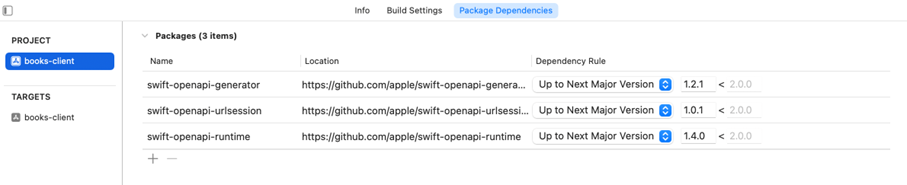
\includegraphics[scale=1.0]{../images/dependencies.png}
    \caption{Dependencies}
    
\end{figure}
\begin{figure}[htbp]
    \centering
    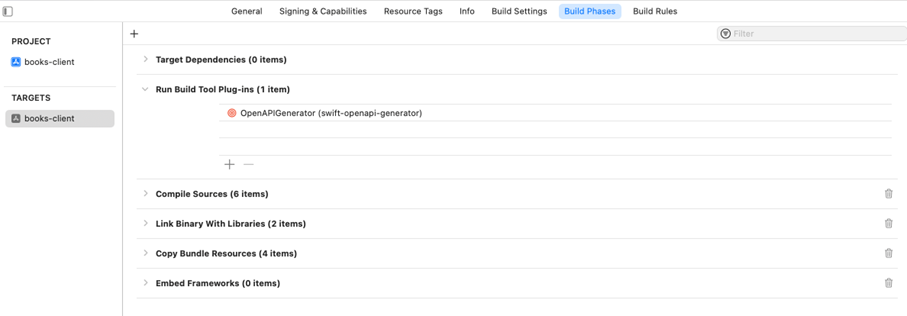
\includegraphics[scale=1.0]{../images/target.png}
    \caption{Run Build Tool Plug-ins}
    
\end{figure}



\subsubsection{Netwerklaag}
Nu wordt er de netwerklaag toevoeg aan het project. In deze netwerklaag wordt voor elk \textit{endpoint} een specifieke functie gecreëerd. Deze functies fungeren als de brug tussen de applicatie en de externe servers, waardoor communicatie mogelijk wordt via de API-\textit{endpoints}. Het bijzondere aan deze functies is dat er niet veel logica aan toegevoegd hoeft te worden, Veel van het proces wordt automatisch afgehandeld door de \textit{Client}. 
Hoewel de meeste van de logica automatisch wordt afgehandeld, er nog steeds aandacht moet worden besteed aan bepaalde aspecten, zoals \textit{error handling}. 

\begin{lstlisting}[caption=ApiService file]
import Foundation
import OpenAPIURLSession

class ApiService<C: APIProtocol> {
    let client : C
    
    init(client: C) {
        self.client = client
    }
    init() where C == Client {
        self.client = Client(
        serverURL: try! Servers.server1(),
        transport: URLSessionTransport()
        )
    }
    
    func getAllBooks() async -> [Components.Schemas.Book] {
        guard let response = try? await client.getAllBooks(Operations.getAllBooks.Input()) else {
            print("Error getting response")
            return []
        }
        
        switch response {
            case .ok(let okResponse):
            switch okResponse.body {
                case .json(let booksResponse):
                return booksResponse
            }
            case .undocumented(statusCode: let statusCode, _):
            print("Undocumented Error: \(statusCode)")
            return []
        }
    }
    
    func createBooks(book: Components.Schemas.Book) async -> Components.Schemas.Book {
        guard let response = try? await client.createBook(.init(body: .json(book))) else {
            print("Error getting response")
            return Components.Schemas.Book(id: "", title: "", author: "")
        }
        
        switch response {
            case .created(let okResponse):
            switch okResponse.body {
                case .json(let booksResponse):
                return booksResponse
            }
            case .undocumented(statusCode: let statusCode, _):
            print("Undocumented Error: \(statusCode)")
            return Components.Schemas.Book(id: "", title: "", author: "")
            case .badRequest(_):
            print("Bad Request")
            return Components.Schemas.Book(id: "", title: "", author: "")
        }
    }
    
    func updateBook(id: String, book: Components.Schemas.Book) async -> Components.Schemas.Book {
        guard let response = try? await client.updateBook(path: .init(id: id), body: .json(book)) else {
            print("Error getting response")
            return Components.Schemas.Book(id: "", title: "", author: "")
        }
        
        switch response {
            case .ok(let okResponse):
            switch okResponse.body {
                case .json(let booksResponse):
                return booksResponse
            }
            case .undocumented(statusCode: let statusCode, _):
            print("Undocumented Error: \(statusCode)")
            return Components.Schemas.Book(id: "", title: "", author: "")
            
        }
    }
    func getById(id: String) async -> Components.Schemas.Book {
        guard let response = try? await client.getById(path: .init(id: id)) else {
            print("Error getting response")
            return Components.Schemas.Book(id: "", title: "", author: "")
        }
        
        switch response {
            case .ok(let okResponse):
            switch okResponse.body {
                case .json(let booksResponse):
                return booksResponse
            }
            case .undocumented(statusCode: let statusCode, _):
            print("Undocumented Error: \(statusCode)")
            return Components.Schemas.Book(id: "", title: "", author: "")
            
            case .notFound(_):
            print("Not Found Error")
            return Components.Schemas.Book(id: "", title: "", author: "")
        }
    }
    
}

\end{lstlisting}

\subsubsection{Het creëren van de views}
Wanneer je netwerk laag gemaakt is, is zeer gemakkelijk om deze functies te gaan verwerken in je views. 

\begin{lstlisting}[caption=ApiService file]
struct ContentView: View {
    @State var BooksData = [Components.Schemas.Book]()
    @Environment(\.dismiss) var dismiss
    @State private var showAddBook = false
    var body: some View {
        VStack {
            NavigationView {
                List {
                    ForEach(BooksData, id: \.id) { book in
                        NavigationLink(destination: BookView(id: book.id)) {
                            Text("\(book.title) - \(book.author)")
                        }
                    }
                }.navigationTitle("Books")
                .toolbar {
                    Button {
                        showAddBook = true
                    }label: {
                        Label("add hotspot", systemImage: "plus.circle")
                    }
                }
            }
        }
        .onAppear{
            Task {
                BooksData = await ApiService().getAllBooks()
            }
        }.sheet(isPresented: $showAddBook, onDismiss: {
            Task {
                BooksData = await ApiService().getAllBooks()
            }
        }) {
            CreateBooks()
        }
    }
}

    
\end{lstlisting}
 \newpage
\section{Scenario 5: aanpasbaarheid van back-end}
Dit scenario wordt geïmplementeerd omdat het eventueel kan zijn dat er nog aanpassingen moeten gebeuren aan de back-end, nadat een \textit{client} is ontwikkeld. 
Specifiek in dit geval zou dat kunnen zijn om bijvoorbeeld extra gegevens toe te voegen aan een boek, namelijk beschrijving, \textit{genre}, … . 


\subsection{Technische doelstellingen}
Hoewel dit scenario niet bijzonder ingewikkeld is, is het cruciaal voor het onderzoeken van de flexibiliteit van een back-end die gebouwd is met de Swift OpenAPI-generator. Deze moet in staat zijn om veranderingen in het OpenAPI-document te accommoderen. Bijvoorbeeld, als er een nieuwe \textit{client} aan het systeem wordt toegevoegd, kunnen er wijzigingen in het OpenAPI-document nodig zijn om nieuwe eisen en functionaliteiten te weerspiegelen. Dit kan variëren van het toevoegen van nieuwe \textit{endpoints} tot het wijzigen van bestaande API-specificaties.

Het is belangrijk om te evalueren hoe flexibel en aanpasbaar de back-end is bij het omgaan met dergelijke veranderingen. Dit omvat de mogelijkheid om snel en efficiënt updates door te voeren in de back-end code en het waarborgen van consistentie en compatibiliteit tussen de OpenAPI-specificaties en de daadwerkelijke implementatie van de API-functionaliteit.

\subsubsection{Aanpasbaarheid back-end}
Het aanpassen van de back-end gaat zeer vlot, Er kunnen gemakkelijk wijzigingen gedaan worden aan het OpenAPI-document en kunnen gemakkelijk verwerkt worden in de \textit{handler}. Belangrijk om op te merken is dat de model en \textit{migration} niet mag vergeten aan te passen. Zo zijn er twee extra \textit{properties}  toegevoegd, namelijk \textit{genre} en beschrijving. 

\begin{lstlisting}[caption=openapi.yaml file]
components:
  schemas:
    Book:
      type: object
      properties:
        id:
          type: string
          format: uuid
          description: The ID of the book
        title:
          type: string
          description: The title of the book
        author:
          type: string
          description: The author of the book
        genre:
          type: string
          items:
            $ref: '#/components/schemas/Genre'
        description:
          type: string
      required:
        - id
        - title
        - author
        - genre
        - description
Genre:
  type: object
  properties:
    name:
      type: string
\end{lstlisting}

\begin{lstlisting}[caption=handler file]
struct Handler: APIProtocol {
    ……    
    func getAllBooks(_ input: Operations.getAllBooks.Input) async throws -> Operations.getAllBooks.Output {
        let books = try await Book.query(on: app.db).all()
        logger.info("successfull GET-request to database")
        
        var booksArray: Array<Components.Schemas.Book> = []
        books.forEach { book in
            booksArray.append(Components.Schemas.Book(id: "\(String(describing: book.id))", title: book.title, author: book.author, genre: book.genre.rawValue, description: book.description))
        }
        logger.info("Converted books of database to return object")
        return .ok(.init(body: .json(booksArray)))
    }
    
    func getById(_ input: Operations.getById.Input) async throws -> Operations.getById.Output {
        let id = UUID(uuidString: input.path.id)
        guard let book = try await Book.find(id, on: app.db) else {
            logger.debug("Can't find Book in database!")
            throw Abort(.notFound)
        }
        
        return .ok(.init(body: .json(Components.Schemas.Book(id: "\(String(describing: book.id))", title: book.title, author: book.author, genre: book.genre.rawValue, description: book.description))))
        
    }
    
    
    func createBook(_ input: Operations.createBook.Input) async throws -> Operations.createBook.Output {
        guard case .json(let bookInput) = input.body else {
            logger.debug("Something went wrong with the Input.body")
            fatalError()
        }
        
        let id = UUID(uuidString: bookInput.id)
        
        //validations of book
        if (bookInput.title.isEmpty || bookInput.author.isEmpty) {
            throw Abort(.badRequest, reason: "Invalid title or author")
        }
        
        var book = Book(id: id, title: bookInput.title, author: bookInput.author, genre: Genre(rawValue: bookInput.genre) ?? Genre.Roman, description: bookInput.description)
        try await book.save(on: app.db)
        
        let bookapi: Components.Schemas.Book
        switch input.body {
            case .json(let json): bookapi = json
            case .none:
            bookapi = .init(id: "", title: "", author: "", genre: "", description: "")
            break
        }
        
        return .created(.init(body: .json(bookapi)))
    }
    
    func updateBook(_ input: Operations.updateBook.Input) async throws -> Operations.updateBook.Output {
        guard case .json(let bookInput) = input.body else {
            logger.debug("Something went wrong with the Input.body")
            fatalError()
        }
        //validations of book
        if (bookInput.title.isEmpty || bookInput.author.isEmpty) {
            throw Abort(.badRequest, reason: "Invalid title or author")
        }
        
        let id = UUID(uuidString: bookInput.id)
        guard let bookDb = try await Book.find(id, on: app.db) else {
            throw Abort(.notFound)
        }
        bookDb.id = UUID(uuidString: bookInput.id)
        bookDb.title = bookInput.title
        bookDb.author = bookInput.author
        bookDb.genre = Genre(rawValue: bookInput.genre) ?? Genre.Roman
        bookDb.description = bookInput.description
        
        try await bookDb.update(on: app.db)
        
        let updatedBook: Components.Schemas.Book
        switch input.body {
            case .json(let json): updatedBook = json
            case .none:
            updatedBook = .init(id: "", title: "", author: "", genre:"", description: "")
            break
        }
        return .ok(.init(body: .json(updatedBook)))
    }
    ………
    
}

\end{lstlisting}

\subsubsection{Aanpasbaarheid front-end}
Het aanpassen van de front-end gaat ook zeer vlot.Belangrijk om op te merken is dat het OpenAPI-document overeenkomt met dat in de back-end. Hierna moet de netwerklaag nog aangepast worden naar de \textit{endpoints} of nieuwe gegevens van de \textit{components}, dit is enkel de \textit{error handling}. En dan kan gestart worden met het verwerken van de nieuwe gegevens in de UI.

\begin{lstlisting}[caption=ApiService file]
class ApiService<C: APIProtocol> {
    let client : C
    
    init(client: C) {
        self.client = client
    }
    init() where C == Client {
        self.client = Client(
        serverURL: try! Servers.server1(),
        transport: URLSessionTransport()
        )
    }
    
    func getAllBooks() async -> [Components.Schemas.Book] {
        guard let response = try? await client.getAllBooks(Operations.getAllBooks.Input()) else {
            print("Error getting response")
            return []
        }
        
        switch response {
            case .ok(let okResponse):
            switch okResponse.body {
                case .json(let booksResponse):
                return booksResponse
            }
            case .undocumented(statusCode: let statusCode, _):
            print("Undocumented Error: \(statusCode)")
            return []
        }
    }
    
    func createBooks(book: Components.Schemas.Book) async -> Components.Schemas.Book {
        guard let response = try? await client.createBook(.init(body: .json(book))) else {
            print("Error getting response")
            return Components.Schemas.Book(id: "", title: "", author: "", genre: "", description: "")
        }
        
        switch response {
            case .created(let okResponse):
            switch okResponse.body {
                case .json(let booksResponse):
                return booksResponse
            }
            case .undocumented(statusCode: let statusCode, _):
            print("Undocumented Error: \(statusCode)")
            return Components.Schemas.Book(id: "", title: "", author: "", genre: "", description: "")
            case .badRequest(_):
            print("Bad Request")
            return Components.Schemas.Book(id: "", title: "", author: "", genre: "", description: "")
        }
    }
    
    func updateBook(id: String, book: Components.Schemas.Book) async -> Components.Schemas.Book {
        guard let response = try? await client.updateBook(path: .init(id: id), body: .json(book)) else {
            print("Error getting response")
            return Components.Schemas.Book(id: "", title: "", author: "", genre: "", description: "")
        }
        
        switch response {
            case .ok(let okResponse):
            switch okResponse.body {
                case .json(let booksResponse):
                return booksResponse
            }
            case .undocumented(statusCode: let statusCode, _):
            print("Undocumented Error: \(statusCode)")
            return Components.Schemas.Book(id: "", title: "", author: "", genre: "", description: "")
            
        }
    }
    func getById(id: String) async -> Components.Schemas.Book {
        guard let response = try? await client.getById(path: .init(id: id)) else {
            print("Error getting response")
            return Components.Schemas.Book(id: "", title: "", author: "", genre: "", description: "")
        }
        
        switch response {
            case .ok(let okResponse):
            switch okResponse.body {
                case .json(let booksResponse):
                return booksResponse
            }
            case .undocumented(statusCode: let statusCode, _):
            print("Undocumented Error: \(statusCode)")
            return Components.Schemas.Book(id: "", title: "", author: "", genre: "", description: "")
            
            case .notFound(_):
            print("Not Found Error")
            return Components.Schemas.Book(id: "", title: "", author: "", genre: "", description: "")        }
    }
    
}

\end{lstlisting}